\subsection{Arrows}
\begin{frame}[fragile]{Arrow Definition (1)}
\centering Another way to think about computations:
\begin{center}
	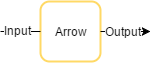
\includegraphics[scale=0.8]{images/arrow}~\\
\end{center}
\end{frame}

\begin{frame}[fragile]{Arrow Definition (2)}
\begin{minipage}{0.6\textwidth}
\begin{lstlisting}[frame=htrbl, numbers=none]
class Arrow arr where
	arr :: (a -> b) -> arr a b
	
	
	
	(>>>) :: arr a b -> arr b c -> arr a c
	
	
	
	
	first :: arr a b -> arr (a,c) (b,c)
\end{lstlisting}
\vfill
\end{minipage}
\hspace*{0.03\textwidth}
\begin{minipage}{0.25\textwidth}
	~\\~\\~\\
	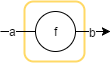
\includegraphics[scale=0.6]{images/arr}~\\~\\
	\includegraphics[scale=0.6]{images/compose}~\\~\\
	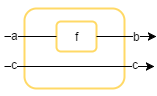
\includegraphics[scale=0.6]{images/first}~\\~\\
\end{minipage}
\end{frame}

\begin{frame}[fragile]{Functions $\in$ Arrows}
Functions \lstinline{(->)} are arrows:
\begin{lstlisting}[frame=htrbl]
instance Arrow (->) where
	arr f = f
	f >>> g = g . f
	first f = \(a, c) -> (f a, c)
\end{lstlisting}
\end{frame}

\begin{frame}[fragile]{The Kleisli Type}
The Kleisli type
\begin{lstlisting}[frame=htrbl]
data Kleisli m a b = Kleisli { run :: a -> m b }
\end{lstlisting}
is also an arrow:
\begin{lstlisting}[frame=htrbl]
instance Monad m => Arrow (Kleisli m) where
	arr f = Kleisli $ return . f
	f >>> g = Kleisli $ \a -> f a >>= g
	first f = Kleisli $ \(a,c) -> f a >>= \b -> return (b,c)
\end{lstlisting}
\end{frame}

\begin{frame}[fragile]{Combinators}
\begin{lstlisting}[frame=htrbl]
(***) :: arr a b -> arr c d ->	arr (a, c) (b, d)
f *** g = first f >>> second g
\end{lstlisting}
\begin{center}
	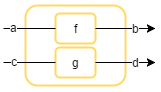
\includegraphics[scale=0.6]{images/starstarstar}
\end{center}
\begin{lstlisting}[frame=htrbl]
(&&&) :: arr a b -> arr a c -> arr a (b, c)
f &&& g = arr (\a -> (a, a)) >>> (f *** g)
\end{lstlisting}
\begin{center}
	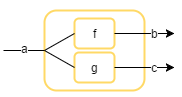
\includegraphics[scale=0.6]{images/dollardollardollar}
\end{center}
\end{frame}

\begin{frame}[fragile]{Arrow Example}
	Arrow usage example:
\begin{lstlisting}[frame=htrbl]
add :: Arrow arr => arr a Int -> arr a Int -> arr a Int
add f g = (f &&& g) >>> arr (\(u, v) -> u + v)
\end{lstlisting}
	\begin{center}
		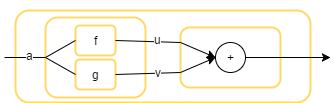
\includegraphics[scale=0.6]{images/addA-comb}
	\end{center}
\end{frame}